\section{SHG-OR}\label{sec:appendix:AdditionalHelixOR}

\subsection{74 nm separated helices}
Figures~\ref{fig:results:OAinPlanarNanohelices:b_s_data} and~\ref{fig:results:OAinPlanarNanohelices:b_p_data} were obtained following the same procedures described in section~\ref{sec:results:OAinPlanarNanohelices}. The structures here were designed to be identical to those in section~\ref{sec:results:OAinPlanarNanohelices}, but with a larger centre-to-centre inclusion separation of $\SI{74}{\nano\m}$. All geometric parameters are given in the  figures.

Notably, neither the data for p-polarised or s-polarised illumination closely match the data shown in section~\ref{sec:results:OAinPlanarNanohelices}. This strongly suggests that the effective susceptibility tensor component values of the metamaterial are strongly dependent on the inclusion separation, even for only slightly different separations well below the operating wavelength. Optical rotation is still observed in both cases, however neither figures~\ref{fig:results:OAinPlanarNanohelices:b_s_data} nor~\ref{fig:results:OAinPlanarNanohelices:b_p_data} show rotation solely attributable to chirality, or clearly dominated by anisotropy.

\subsection{$1.5 \times$ scaled helices}
Figures~\ref{fig:results:OAinPlanarNanohelices:8_s_data} and~\ref{fig:results:OAinPlanarNanohelices:8_p_data} were obtained following the same procedures described in section~\ref{sec:results:OAinPlanarNanohelices}. The structures here are designed to be $\approx 1.5 \times$ scaled copies of those in section~\ref{sec:results:OAinPlanarNanohelices}. In practice, this is difficult to achieve. Notably, the wire thickness is the same as in section~\ref{sec:results:OAinPlanarNanohelices}, and while the height is indeed $1.5 \times$ scaled, the helical pitch and inclusion separation are closer to $1.3 \times$.  Nevertheless, this data demonstrates the effect of changing the geometry of the nanohelix structures themselves. All geometric parameters are given in the  figures.

Interestingly, figure~\ref{fig:results:OAinPlanarNanohelices:8_p_data} shows behaviour qualitatively very similar to that in figure~\ref{fig:results:OAinPlanarNanohelices:p_data}. These larger helices exhibit the same anisotropy-dominated optical rotation for p-polarised incident light, however the behaviour under s-polarised illumination is dramatically different to section~\ref{sec:results:OAinPlanarNanohelices}. The similarity in behaviour under p-polarised illumination suggests that the effective susceptibility tensor values are less sensitive to changes in the individual inclusion dimensions than the arrangement and separation of the inclusions.

In both figures~\ref{fig:results:OAinPlanarNanohelices:b_s_data} and~\ref{fig:results:OAinPlanarNanohelices:8_s_data}, the rotation of s-polarised incident light cannot be solely attributed to the structural chirality, due to both strong angular variations, and a lack of inversion between enantiomorphs. This demonstrates the ``Goldilocks'' nature of the effect observed in section~\ref{sec:results:OAinPlanarNanohelices}, whereby the interaction of particular susceptibility tensor component values allows the direct measurement of intrinsic structural chirality, under particular experimental conditions.

\begin{figure}[htb]	
    \centering	
    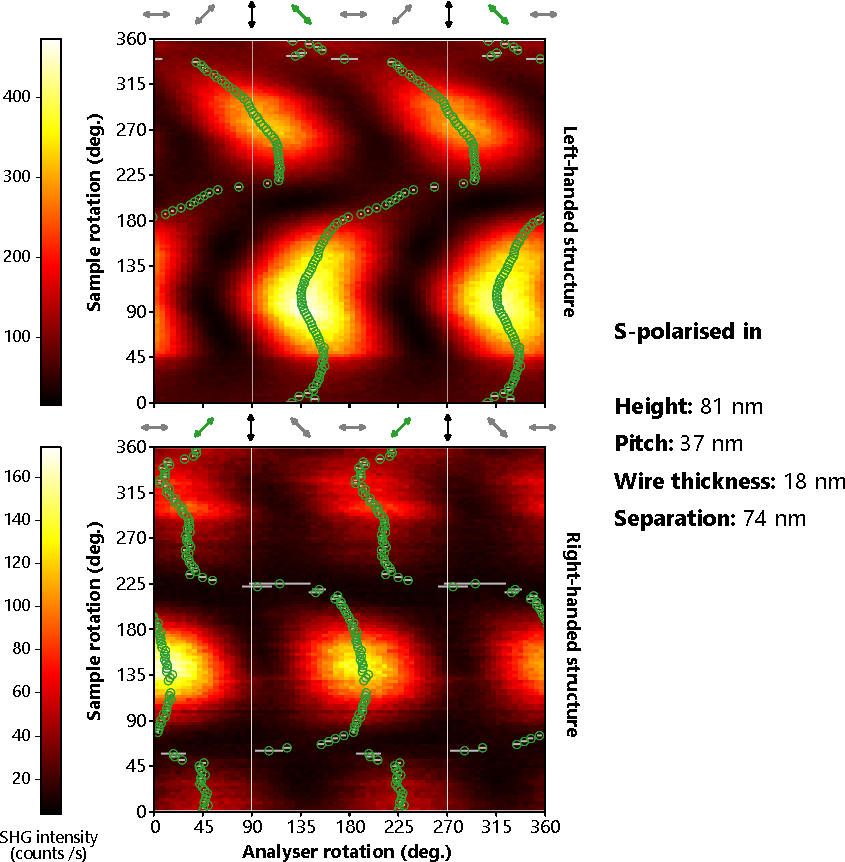
\includegraphics[scale=1]{./figures/results/OAinPlanarNanohelices/b_s_data.pdf}
    \caption{\label{fig:results:OAinPlanarNanohelices:b_s_data}
    SHG optical rotation heatmaps for helical metamaterial, with $\SI{74}{\nano\m}$ inclusion separation, for S-polarized incident light.}	
\end{figure}

\begin{figure}[htb!]	
    \centering	
    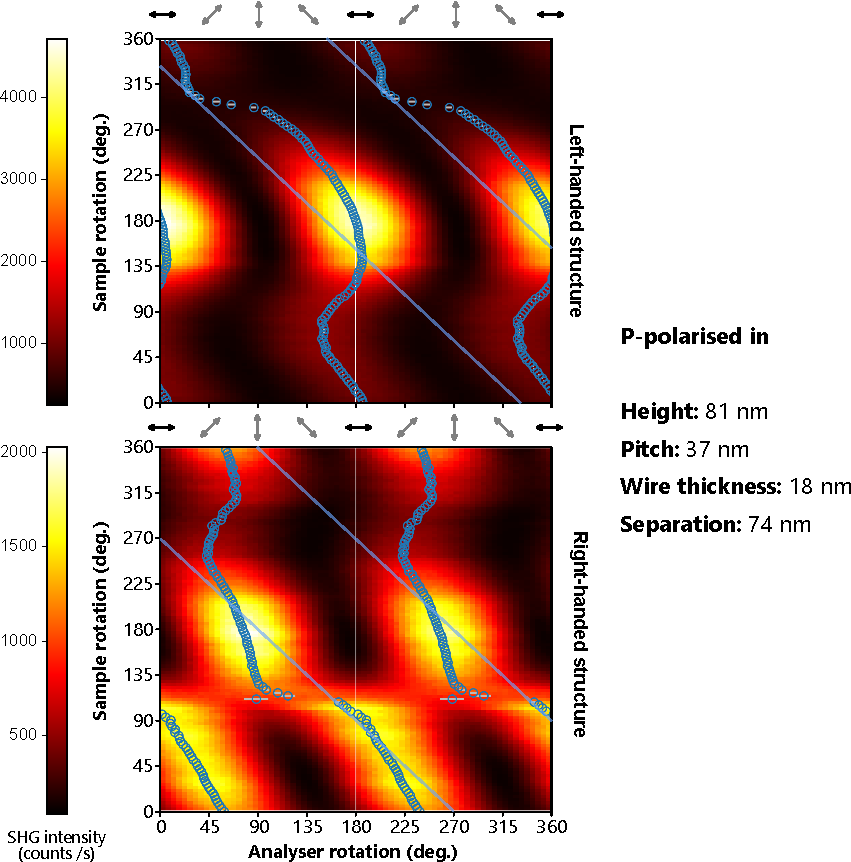
\includegraphics[scale=1]{./figures/results/OAinPlanarNanohelices/b_p_data.pdf}

    \caption{\label{fig:results:OAinPlanarNanohelices:b_p_data}
    SHG optical rotation heatmaps for helical metamaterial, with $\SI{74}{\nano\m}$ inclusion separation, for P-polarized incident light.}	
\end{figure}

\begin{figure}[htb!]	
    \centering	
    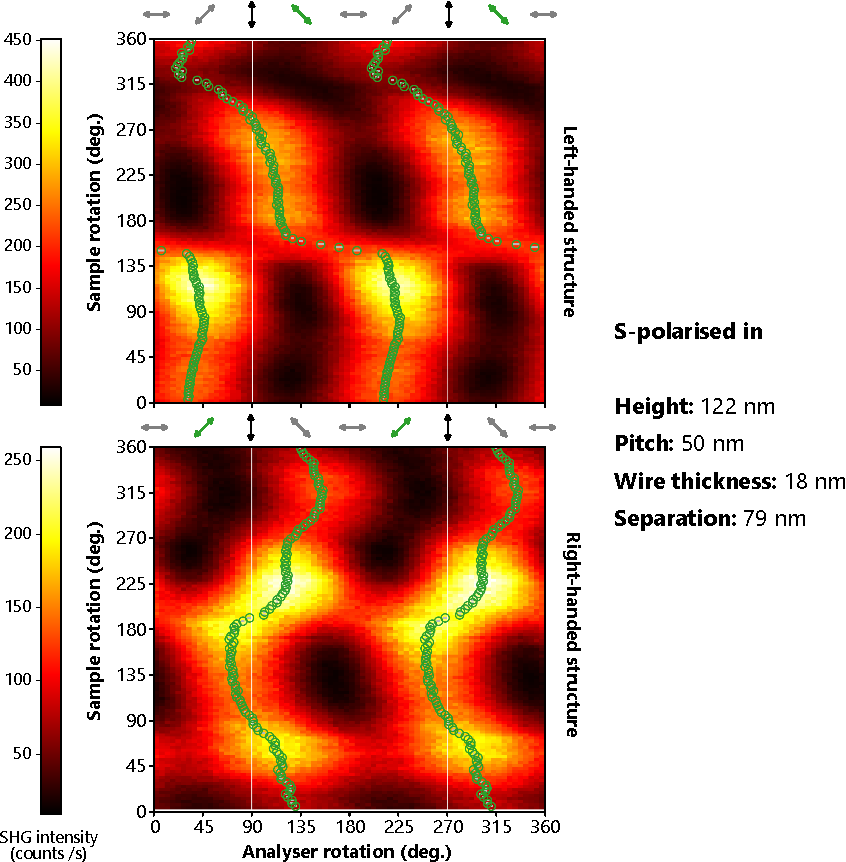
\includegraphics[scale=1]{./figures/results/OAinPlanarNanohelices/8_s_data.pdf}
    \caption{\label{fig:results:OAinPlanarNanohelices:8_s_data}
    SHG optical rotation heatmaps for helical metamaterial, with $\SI{122}{\nano\m}$ height, $\SI{50}{\nano\m}$ pitch, $\SI{18}{\nano\m}$ wire thickness, and $\SI{79}{\nano\m}$ inclusion separation, for S-polarized incident light.}	
\end{figure}

\begin{figure}[htb!]	
    \centering	
    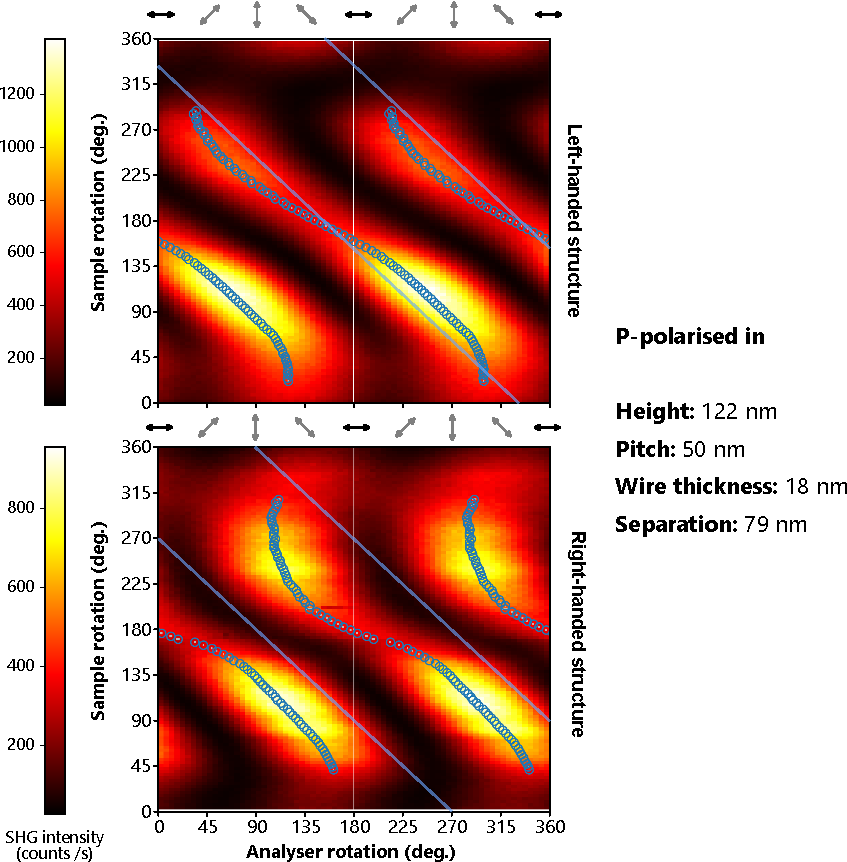
\includegraphics[scale=1]{./figures/results/OAinPlanarNanohelices/8_p_data.pdf}

    \caption{\label{fig:results:OAinPlanarNanohelices:8_p_data}
    SHG optical rotation heatmaps for helical metamaterial, with $\SI{122}{\nano\m}$ height, $\SI{50}{\nano\m}$ pitch, $\SI{18}{\nano\m}$ wire thickness, and $\SI{79}{\nano\m}$ inclusion separation, for P-polarized incident light.}	
\end{figure}